\title{RADseq Works in Primates, Dammit.}
\author{
        Christina M. Bergey
			\and
			Luca Pozzi
			\and
			Todd R. Disotell
			\and
			Andrew S. Burrell
	}
\date{\today}

\documentclass[12pt]{article}

\usepackage{color}
\usepackage{graphics}

\begin{document}
\maketitle

\begin{abstract}
\textcolor{red}{\ldots (This is just a bit of the blurb from the email.) Our paper is an introduction to a 2nd generation sequencing technique for typing thousands of genome-wide markers from non-model organisms.  We demonstrate it in five primates and discuss its promise for doing mutli-locus phylogenetics and population genetics in primates. \ldots}
\end{abstract}

\section{Introduction}

During the first decades of molecular primatology, a formidable impediment to researchers was the need to develop and type polymorphic markers in a taxon of interest. The markers that resulted from this tedious and expensive task were often uninformative when applied outside of the population used in their design, necessitating further rounds of primer design or microsatellite assays, for example (Davey et al., 2011). Due to the bottleneck of marker discovery, many population genetic or phylogenetic studies in molecular primatology have been based on one or few loci (\textcolor{red}{Ting and Sterner, published yet?}). Such inferences can reliably give the evolutionary history of those particular regions of the genome, but they fail to adequately capture the complete complex history of the population given the mosaic nature of genomic evolution (\textcolor{red}{some gene-tree species tree review ref}). Adequate resolution depends on high marker density, and until recently that goal has been out of reach for many primate researchers.

The rapidly decreasing costs of DNA sequencing technology have promised revolutionary gains for primatology (\textcolor{red}{Enard and Paabo 2004, maybe? Goodman et al 2005?}). A primate researcher benefits from the many nearby sequenced and assembled reference genomes in the order, but genomic studies of non-model organisms nevertheless remain difficult. Though the cost of low coverage whole genome sequencing has fallen to a level feasible for many researchers' budgets, sequencing whole genomes for the tens or hundreds of individuals desired in a typical population genetic study is often prohibitively expensive and quite possibly superfluous. 

Fortunately, researchers have recently developed techniques that reduce the complexity of the genome and allow discovery and typing of thousands or tens of thousands of genome-wide makers in many individuals in a single step. RAD-seq is one such simple, inexpensive reduced representation technique which allows for the sequencing of small fragments of the genome adjacent to restriction enzyme cut sites (Baird et al., 2008). These RAD tags, or restriction-site association DNA tags, were originally developed for use in microarray hybridization typing (Miller et al., 2007), but an updated protocol substitutes second-generation DNA sequencing to rapidly discover and type SNPs (Baird et al., 2008). The lack of reliance on a reference genome and applicability to datasets of many individuals make it a promising technique for phylogenetic or population genetic studies in non-model organisms, such as many primates.

In the present study, we summarize the RAD-seq method in brief and note the many and varied applications since its development. We go on to discuss reasons that make RAD-seq promising for primatologists, and then demonstrate the technique in 5 primates: a lemur, New World monkey, Old World monkey, and two apes.  

\subsection{The RAD-seq Technique}

The following is a summary of the RAD tag library preparation of Etter et al., 2011 (\textcolor{red}{Fig. 1}). The RAD-seq library preparation begins when genomic DNA from multiple individuals is digested with a restriction enzyme, such as \emph{EcoRI} or \emph{PspXI}. The P1 adapter is then ligated to the fragments, connected to the sticky end at the restriction enzyme cut site. The P1 adapter contains an amplification site for PCR, an Illumina sequencing priming site, and an individual-specific barcode of five basepairs. Once the barcode has been added, fragments from multiple individuals can be pooled, and the DNA is randomly sheared with a sonicator to have a length distribution under 1 kilobase. To select for reads that are suitable for sequencing on the Illumina platform, the sheared samples are size selected via agarose gel electrophoresis, extracting fragments between 300 and 500 bp in length. The second adapter, P2, is a Y adapter meaning its two halves are complementary for only part of their length. It is ligated to the fragments and then the fragments are amplified via PCR. Because the second adapter has divergent ends, the reverse amplification primer is unable to bind until after the forward amplification primer has filled in its complementary sequence. This ensures that only RAD tags ligated to P1 are able to amplify. After few cycles of PCR to minimize the risk of introducing PCR artifacts or biases, the library is ready for final clean-up, quality control, and sequencing.

\subsection{Previous RAD-seq Studies}

\textcolor{red}{[Previous RADseq studies. Focus on pop gen, phylogeny studies]}

\subsection{Prospective Primate Applications}

\textcolor{red}{[Why it would be good in primates.]}

Changing the restriction enzyme to a more or less frequent cutter allows fine grained control over the number of loci, number of individuals multiplexed, and depth of coverage, allowing researchers to tailor marker discovery to their hypothesis. 

\section{Methods}

\paragraph{Library Preparation and Sequencing}

	We digested genomic DNA from 5 primates with \emph{PspXI} (New England Biolabs) and used it to create a multiplexed RAD tag library. Our library preparation method followed that of Etter et al, 2011 with the following modifications: the P1 adapter top\textcolor{red}{(?)} oligonucleotide was modified to have an overhang corresponding to the cut site of \emph{PspXI}, and a longer P2 adapter suitable for paired end sequencing was used (P2\_top: 5'-\textcolor{red}{SEQUENCEHERE}-3'; P2\_bottom: 5'-\textcolor{red}{SEQUENCEHERE}-3'). Individual-specific barcodes contained in the P1 adapter differed by at least \textcolor{red}{three} nucleotides. We chose \emph{PspXI} based on the results of \emph{in silico} digestion of the human, rhesus macaque, and baboon reference genomes using custom Perl scripts (\textcolor{red}{refs}). We sequenced the prepared library as one 150-cycle paired-end run of an Illumina MiSeq at the NYU Langone Medical Center's Genome Technology Center using a spike-in of 30\% PhiX DNA to control for low diversity in the library at the barcode and restriction sites. Other individuals were sequenced alongside those of the present study. Sequences are available to download from the NCBI Short Read Archive (accession number \textcolor{red}{SRAXXXXXX.X}).

\paragraph{Sequence Analysis - Clustering and SNP Discovery}

We demultiplexed, or separated by barcode, sequence reads and excluded from the analysis reads without an expected barcode or an intact restriction enzyme cut site. We also removed reads with any quality scores below 10. Using the program Stacks, we clustered all reads into matching sets and compared closely related sets to detect orthologous loci and SNPs using a maximum likelihood approach (\textcolor{red}{Stacks ref}). We tallied orthologous SNPs using VCFtools (\textcolor{red}{ref}).

\textcolor{red}{[Phylogeny?]}

\paragraph{Sequence Analysis - Assess RAD Tag Coverage}

To assess the RAD tag coverage, we mapped human and chimpanzee reads to the human reference genome. Again, we excluded reads without an expected barcode or an intact restriction enzyme cut site. We aligned reads to the human reference genome (\textcolor{red}{hg19, ref}) using BWA with default parameters. We removed reads that were unmapped or that had low mapping quality after alignment using Picard (\textcolor{red}{ref}) and BamTools (\textcolor{red}{ref}). 

\textcolor{red}{Cut this paragraph?} After performing local realignment around indels with GATK (\textcolor{red}{ref}), we identified SNPs and short indels using SAMtools mpileup and BCFtools (\textcolor{red}{ref}). We required a minimum coverage of 3 reads and a maximum of 100 to call a SNP or an indel at a given location. We tallied orthologous SNPs using VCFtools (\textcolor{red}{ref}).
	
To assess how many restriction sites were successfully sequenced and to analyze the degree of overlap between multiplexed individual's datasets, we first found all possible \emph{PspXI} cut sites in the human genome using the oligoMatch utility in the USCS Genome Browser program (\textcolor{red}{ref}). This allowed us to calculate the coverage of these restriction site-associated regions using BEDtools' multiBamCov program (\textcolor{red}{ref}).

\section{Results}

% 3804227030 bp total (12,983,710 pairs of reads * (142bp + 151bp). This includes non-OWM taxa, remember.
% OWM sequencing reads: 6,125,860 total, half that many pairs
% Of those, 2029586 passed the filtration steps

\_\_\_ million sequencing reads with an intact barcode and restriction enzyme cut site could be assigned confidently to one of the five primates in the present study. Roughly \_\_\_ million of those reads passed quality control filtration and \_\_\_ could be assigned to a stack. In these stacks our study identified \_\_\_ SNPs among all samples. Information for each individual is summarized in Table 1. 

\begin{table}[h]
\caption{Clustered Reads Data}
\begin{center}
	\small
	\begin{tabular}{ p{3cm} || l || p{1.75cm} | p{1.75cm} || p{1.75cm} | p{1.75cm} | l }
		\hline
		Taxon & Source & \# Reads & \# Filtered Reads & \# Stacks & Mean Coverage & \# SNPs \\ \hline\hline
		\emph{Microcebus \textcolor{red}{murinus?}} & \textcolor{red}{Unknown} &  &  &  &  &  \\ \hline
		\emph{Cebus \textcolor{red}{sp.?}} & \textcolor{red}{Unknown} &  &  &  &  &  \\ \hline
		\emph{Theropithecus gelada} & \textcolor{red}{Unknown} &  &  &  &  &  \\ \hline
		\emph{Pan troglodytes} & \textcolor{red}{Unknown} &  &  &  &  &  \\ \hline
		\emph{Homo sapiens} & \textcolor{red}{Unknown} &  &  &  &  &  \\ \hline
		\hline
	\end{tabular}
\end{center}
\end{table}

In the human genome, we found \_\_\_ possible cut sites for \emph{PspXI} and \_\_\_ possible sequencing sites (two per cut site, one upstream and one downstream). Of those, \_\_\_ sites (\_\_\_\%) were covered by at least one read in human and \_\_\_ sites (\%) in chimpanzee. For \_\_\_ sites (\_\_\%), both chimpanzee and human had at least one read. When we restrict the analysis to sites with at least three reads, \_\_\_ sites (\_\_\_\%) were covered in human, \_\_\_ sites (\_\_\_\%) were covered in chimpanzee, and \_\_\_ sites (\_\_\_\%) in both.

\begin{table}[h]
\caption{Mapped Reads Data}
\begin{center}
	\small
	\begin{tabular}{ p{3cm} || p{1.75cm} | p{1.75cm} || p{1.75cm} | p{1.75cm} | l }
		\hline
		Taxon & \# Reads & \# Filtered Reads & \# Loci $\ge 1$ Read & \# Loci $\ge 3$ Reads & \# SNPs \\ \hline\hline
		\emph{Pan troglodytes} &  &  &  &  &  \\ \hline
		\emph{Homo sapiens} &  &  &  &  &  \\ \hline
		\hline
	\end{tabular}
\end{center}
\end{table}


%\begin{itemize}
%	\item Pairwise comparisons between individuals? Like X orthologous regions shared between Papio and Thero?
%\end{itemize}
%
%%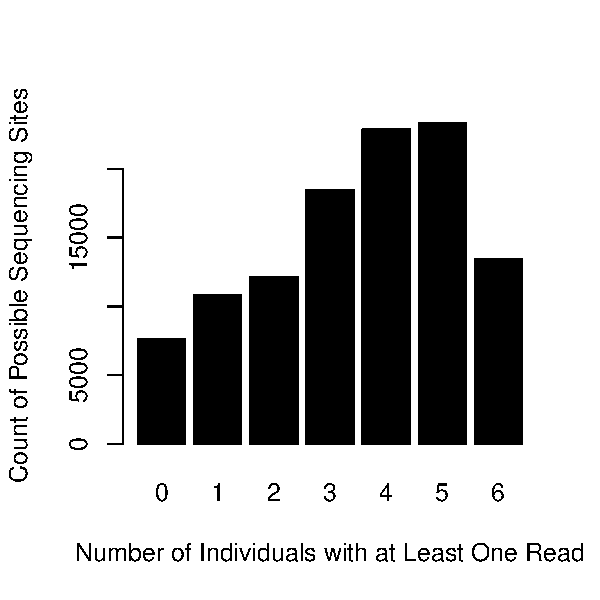
\includegraphics{figs/seq_site_coverage_by_ind}
%
%\begin{itemize}
%	\item SNP info from merged analysis
%	\item SNP Venn diagram?
%	\item Count orthologous SNPs shared between individuals. Pairwise?
%\end{itemize}

\section{Discussion}
\textcolor{red}{
\begin{itemize}
	\item RADseq is viable tool for researcher interested in primate phylogenetics, pop. gen.
	\begin{itemize}
		\item Cheap and easy to create libraries. Competent lab can do it in two days. (Ha!)
		\item Multiplexing is great for pop gen studies.
		\item Enzyme choice allows control over coverage, number of individuals, number of loci.
		\item Baird: "different marker densities can be attained by choice of restriction enzyme"
	\end{itemize}
	\item Potential problems with RADseq method
	\item ddRADseq
	\item Promise for primatology
\end{itemize}
}

\section{Acknowledgements}
\begin{itemize}
	\item NYU Med School folk
	\item \textcolor{red}{Grants?}
\end{itemize}

\end{document}
